
\section{Using R To View Model Output (r4ss)}\label{r4ss}

A collection of functions developed as a package, \texttt{r4ss}, for the statistical software R has been created to explore SS model output.  The functions include tools for summarizing and plotting results, manipulating files, visualizing model parameterizations, and various other tasks.  Currently, information on the code, including installation instructions, can be found at github.com/r4ss/r4ss.  The software package is under constant development to maintain compatibility with new versions of SS and to improve functionality.

Two of the most commonly used functions for model diagnostics are SS\_output and SS\_plots.  After running a model using SS, the report can be read into R by the SS\_output function which stores quantities in a list with named objects.  This list can then be passed to the SS\_plots function which creates a series of over 100 plots that are useful to visualize output such as model fit to the data and time series of quantities of interest.

The latest \texttt{r4ss} version on CRAN can be installed using a command like:

\begin{quote}
	\begin{verbatim}
	> install.packages("r4ss")
	\end{verbatim}
\end{quote}


However, more frequent enhancements and bug fixes are posted to the GitHub project.  The latest version of \texttt{r4ss} can be installed directly from GitHub at any time via the \texttt{devtools} package in R with the following commands:

\begin{quote}
	\begin{verbatim}
	> install.packages("devtools")
	> devtools::install_github("r4ss/r4ss")
	\end{verbatim}
\end{quote}

Note: \texttt{devtools} will give this message: \textit{"WARNING: Rtools is required to build R packages, but is not currently installed."} However, \texttt{Rtools} is NOT required for installing \texttt{r4ss} via \texttt{devtools}, so ignore this warning.

Once you have installed the \texttt{r4ss} package, it can be loaded in the regular manner:

\begin{quote}
	\begin{verbatim}
	> library(r4ss)
	\end{verbatim}
\end{quote}


The results from a model run can be read in and plots created using the following commands:

\begin{quote}
	\begin{verbatim}
	> setwd("C:\directory where model was run")
	> base.model = SS_output(getwd())
	> SS_plots(base.model)
	\end{verbatim}
\end{quote}


\pagebreak
Example of the data displayed used by the SS\_output function:
\begin{center}
		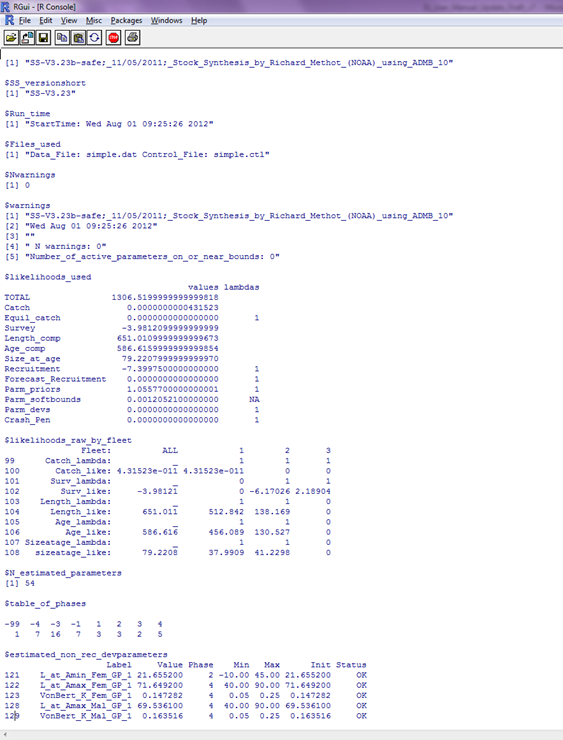
\includegraphics{r4ss_output}
\end{center}

\pagebreak
Example of the plots created using the SS\_plots function:
\begin{center}
	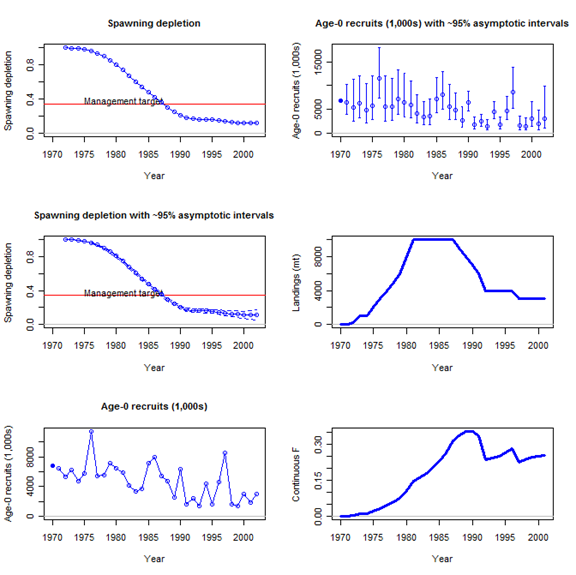
\includegraphics{r4ss_plots}
\end{center}

\pagebreak
The functions included in r4ss ranging from general use to functions developed for specific model applications:
\begin{center}
	\begin{longtable}{p{4.5cm} p{10.52cm}}
		\hline
		Core Functions & \Tstrut\Bstrut\\
		\hline
		SS\_output \Tstrut& A function to create a list object for the output from Stock Synthesis\\
		SS\_plots  \Tstrut& Plot many quantities related to output from Stock Synthesis\\
		\hline
		
		\multicolumn{2}{l}{Plot functions called by SS\_plots:} \Tstrut\Bstrut\\
		\hline
		SSplotBiology \Tstrut& Plot biology related quantities from Stock Synthesis model output, including mean weight, maturity, fecundity, and spawning output. \\
		SSplotCatch   \Tstrut & Plot catch related quantities \\
		SSplotCohorts \Tstrut & Plot cumulative catch by cohort \\
		SSplotComps   \Tstrut & Plot composition data and fits \\
		SSplotData    \Tstrut & Timeline of presence/absence data by type, year, and fleet \\
		SSplotDiscard \Tstrut & Plot fit to discard fraction \\
		SSplotIndices \Tstrut & Plot indices of abundance and associated quantities \\
		SSplotMnwt    \Tstrut & Plot mean weight data and fits \\
		SSplotMovementMap \Tstrut & Show movement rates on a map \\
		SSplotMovementRates \Tstrut & Show movement rates on a map \\
		SSplotNumbers \Tstrut& Plot numbers-at-age related data and fits \\
		SSplotRecdevs \Tstrut& Plot recruitment deviations \\
		SSplotRecdist \Tstrut& Plot of recruitment distribution among areas and seasons \\
		SSplotSelex   \Tstrut& Plot selectivity \\
		SSplotSexRatio \Tstrut& Plot sex ratios \\
		SSplotSummaryF \Tstrut& Plot time series summary of F (or harvest rate) \\
		SSplotSpawnrecruit \Tstrut& Plot spawner-recruit curve \\
		SSplotSPR     \Tstrut& Plot SPR quantities \\
		SSplotTags    \Tstrut& Plot tagging data and fits \\
		SSplotTimeseries \Tstrut& Plot time series data \\
		SSplotYield   \Tstrut& Plot yield and surplus production \\
		SS\_html \Tstrut& Create HTML files to view figures in browser \\
		SS\_fitbiasramp \Tstrut& Estimate bias adjustment for recruitment deviates \Bstrut\\
		\hline
	
		\multicolumn{2}{l}{Model Comparisons and other diagnostics:} \Tstrut\Bstrut\\
		\hline
		SSplotPars    \Tstrut & Plot distributions of priors, posteriors, and estimates \\
		SSplotProfile \Tstrut & Plot likelihood profile results \\
		PinerPlot     \Tstrut & Plot fleet-specific contributions to likelihood profile \\
		SSplotRetroRecruits \Tstrut & Make retrospective pattern of recruitment estimates (a.k.a. squid plot) as seen in Pacific hake assessments\Bstrut \\
		\hline
		
		\multicolumn{2}{l}{Functions related to MCMC diagnostics:}\Tstrut\Bstrut\\
		\hline
		mcmc\_nuisance \Tstrut & Summarize nuisance MCMC output \\
		mcmc\_out      \Tstrut & Summarize, analyze, and plot key MCMC output \\
		SSgetMCMC      \Tstrut & Read MCMC output \\
		SSplotMCMC\_ExtraSelex \Tstrut & Plot uncertainty around chosen selectivity ogive from MCMC \Bstrut\\
		\hline
		
		\multicolumn{2}{l}{Interactive tools for exploring functional forms:} \Tstrut\Bstrut\\
		\hline
		movepars    \Tstrut  & Explore movement parameterization \\
		selfit      \Tstrut  & A function to visualize parameterization of double normal and double logistic selectivity in SS \\
		selfit\_spline \Tstrut & Visualize parameterization of cubic spline selectivity in SS \\
		sel\_line   \Tstrut & A function for drawing selectivity curves\Bstrut \\
		\hline


		\multicolumn{2}{l}{File manipulation for inputs:}\Tstrut\Bstrut\\
		\hline
		SS\_readdat  \Tstrut & Read data file \\
		SS\_readforecast \Tstrut & Read forecast file \\
		SS\_readstarter  \Tstrut & Read starter file \\
		SS\_writedat  \Tstrut & Write data file \\
		SS\_writeforecast \Tstrut & Write forecast file \\
		SS\_writestarter  \Tstrut & Write starter file \\\Tstrut 
		SS\_makedatlist   \Tstrut & Make a list for SS data \\
		SS\_parlines    \Tstrut & Get parameter lines from SS control file \\
		SS\_changepars  \Tstrut  & Change parameters in the control file \\
		SSmakeMmatrix    \Tstrut & Create inputs for entering a matrix of natural mortality by age and year \\
		SS\_profile      \Tstrut & Run a likelihood profile in SS (incomplete) \\
		NegLogInt\_Fn     \Tstrut& Calculated variances of time-varying parameters using SS implementation of the Laplace Approximation \Bstrut\\
		\hline

		\multicolumn{2}{l}{File manipulations for outputs:}\Tstrut\Bstrut\\
		\hline
		SS\_recdevs  \Tstrut & Insert a vector of recruitment deviations into the control file \\
		SS\_splitdat \Tstrut & Split apart bootstrap data to make input file \Bstrut\\
		\hline

		\multicolumn{2}{l}{Minor plotting functions:}\Tstrut\Bstrut\\
		\hline
		bubble3         \Tstrut & Create a bubble plot \\
		make\_multifig  \Tstrut & Create multi-figure plots \\
		Make\_multifig\_sexratio \Tstrut & Create multi-figure plots of sex ratios \\
		plotCI          \Tstrut & Plot points with confidence intervals \\
		rich\_colors\_short \Tstrut & Make a vector of colors \\
		stackpoly       \Tstrut & Plot stacked polygons \\
		mountains       \Tstrut & Make shaded polygons with a mountain-like appearance \Bstrut\\
		
		\hline
		\multicolumn{2}{l}{Really specialized functions:} \Tstrut\Bstrut\\
		\hline
		DoProjectPlots \Tstrut & Make plots from Rebuilder program \\
		IOTCmove       \Tstrut & Make a map of movement for a 5-area Indian Ocean model \\
		SSFishGraph    \Tstrut & A function for converting SS output to the format used by FishGraph \\
		TSCplot        \Tstrut & Create a plot for the TSC report \Bstrut\\
		\hline
	\end{longtable}
\end{center}
